\documentclass{tufte-handout}

\title{Nine strategies for improving transport}

\author{Dr James Reynolds \\ Public Transport Research Group (PTRG) \\ Monash University}

%\date{28 March 2010} % without \date command, current date is supplied

%\geometry{showframe} % display margins for debugging page layout

\usepackage{graphicx} % allow embedded images
  \setkeys{Gin}{width=\linewidth,totalheight=\textheight,keepaspectratio}
  \graphicspath{{graphics/}} % set of paths to search for images
\usepackage{amsmath}  % extended mathematics
\usepackage{booktabs} % book-quality tables
\usepackage{units}    % non-stacked fractions and better unit spacing
\usepackage{multicol} % multiple column layout facilities
\usepackage{lipsum}   % filler text
\usepackage{fancyvrb} % extended verbatim environments
\usepackage{natbib}
  \fvset{fontsize=\normalsize}% default font size for fancy-verbatim environments

% Standardize command font styles and environments
\newcommand{\doccmd}[1]{\texttt{\textbackslash#1}}% command name -- adds backslash automatically
\newcommand{\docopt}[1]{\ensuremath{\langle}\textrm{\textit{#1}}\ensuremath{\rangle}}% optional command argument
\newcommand{\docarg}[1]{\textrm{\textit{#1}}}% (required) command argument
\newcommand{\docenv}[1]{\textsf{#1}}% environment name
\newcommand{\docpkg}[1]{\texttt{#1}}% package name
\newcommand{\doccls}[1]{\texttt{#1}}% document class name
\newcommand{\docclsopt}[1]{\texttt{#1}}% document class option name
\newenvironment{docspec}{\begin{quote}\noindent}{\end{quote}}% command specification environment

\begin{document}

\maketitle% this prints the handout title, author, and date


\begin{marginfigure}%
  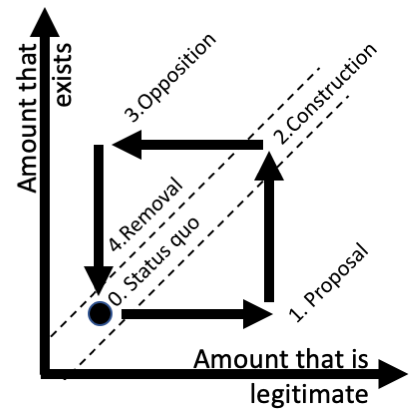
\includegraphics[width=\linewidth]{Framework_and_progression}
  \caption{Legitimacy framework and a simple progression}
  \label{fig:Legitimacy_framework}
\end{marginfigure}
  


\begin{abstract}
\noindent
Why is improving transport so hard? How can bus or bike lanes, pedestrian malls, or other beneficial (but potentially unpopular or controversial) measures be successfully implemented? This handout outlines a new framework (Figure \ref{fig:Legitimacy_framework}) and nine pragmatic strategies, which may help you improve transport systems in the real-world of politics, NIMBYism and other non-technical challenges.
\end{abstract}

\smallcaps{Legitimacy} comes in many forms\footnote{Normative, sociological, through trust, through reasonableness, through unconditional duty, through public consent, or associated with conditional normative support.}, and what is considered legitimate might vary with time or by arena\footnote{For example, installing a bus or bike lane might be identified as the 'best' option in a engineering or planning department, yet be considered unreasonable by drivers, business owners or the local council.}. Figure \ref{fig:Legitimacy_framework} shows a new framework for understanding implementation and changes in what is legitimate.  It shows a simple progression where an improvement is proposed, legitimised and built, but then opposed, delegitimised and removed. Other progressions (Figure \ref{fig:Failure_or_compromise}) might lead to rejection of a proposal entirely or a compromise. For example, a bus lane might be warranted, but opposition might lead to no change from the status quo or a compromise High Occupancy Vehicle (HOV) lane instead. 

\begin{marginfigure}%
  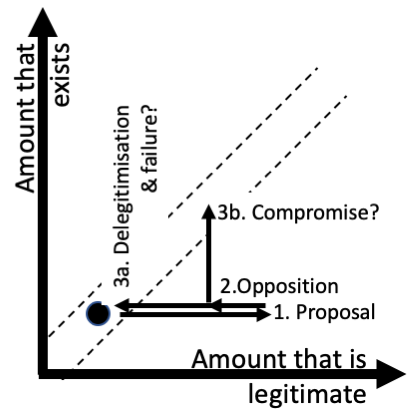
\includegraphics[width=\linewidth]{Failure_or_compromise}
  \caption{Failure or compromise}
  \label{fig:Failure_or_compromise}
\end{marginfigure}




\begin{marginfigure}%
  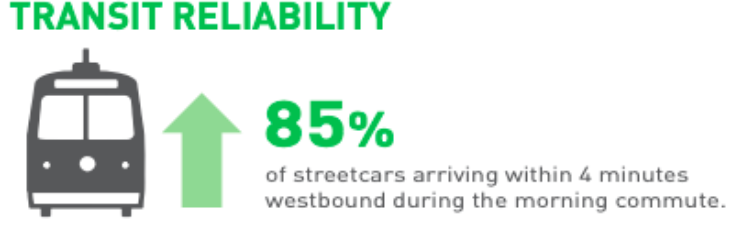
\includegraphics[width=\linewidth]{Toronto_dashboard_1}
   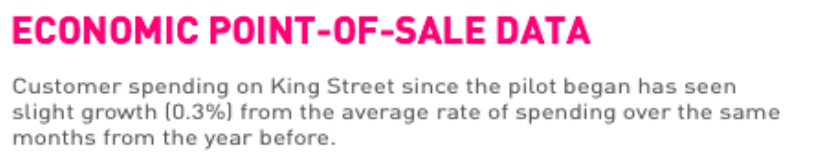
\includegraphics[width=\linewidth]{Toronto_dashboard_4}
  \caption{City of Toronto monthly dashboard during King Street Pilot (excerpt), see thesis p.274}
  \label{fig:Toronto_dashboard}
\end{marginfigure}

\newthought{But how to make progress?} The research described here examined cases of successful and not-as-successful pedestrian malls, bicycle lanes and transit priority measures across Curitiba, Zürich, Boston, Toronto and Melbourne\cite{Reynolds:2020aa}. Emerging from the research was the framework, which helped to explain and identify \smallcaps{Nine Pragmatic Strategies} for legitimising implementation. The first three involve \smallcaps{Building legitimacy} \textbf{BEFORE} implementation. This might involve (A1) \textbf{Technical Reporting}, which is already a typical engineering and planning activity. However, here it is suggested that this be focused towards other, non-technical policy arenas. Figure \ref{fig:Toronto_dashboard} shows an example from Toronto, where monthly dashboards during the King Street Transit Pilot showed data on transit performance, traffic impacts and changes to economic activity in a format tailored for public consumption. A (A2) \textbf{Transport Plan} might also be used, although the research findings suggest that vision-based plans might be more likely to help implementation succeed. For example, Curitiba's famous Bus Rapid Transit (BRT) network was supported by a plan for transport and land-use to develop along linear 'Structural Axes'. Similarly, the Citizens' Transit Priority Initiative in Zürich called for buses and trams to "travel along their lanes or tracks virtually as fast as is technically possible"\cite{Nash:2001ab}. A counter-example is provided by the partially-removed Stud Road bus lanes in Melbourne, where the supporting transport plan set bus lanes as a specific objective\footnote{Rather than a more flexible vision of doing whatever could be done to increase bus speeds and reliability.}. (A3) \textbf{Public Processes} might also be used to build legitimacy, as in Zürich where the Citizens' Transit Priority Initiative was passed in a public ballot, providing legitimacy through public consent. Direct democracy deciding transport policy appears rare, but the research found cases where council meetings, hearings, elections and other public processes helped legitimise implementation.  



\begin{marginfigure}%
  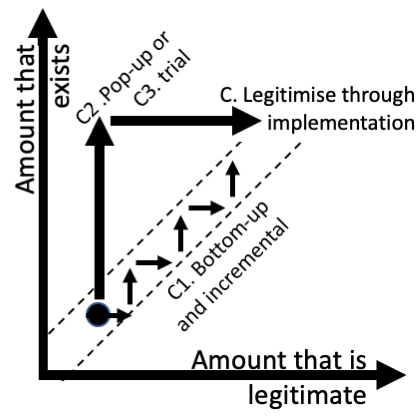
\includegraphics[width=\linewidth]{Figure4}
  \caption{Building legitimacy through implementation}
  \label{fig:FIgure4}
\end{marginfigure}

\newthought{But, why not simply} \textbf{AVOID IMPACTING} those who might oppose implementation?  This approach was successful for the Eglinton Crosstown LRT in Toronto, some of which is (B1) \textbf{Grade-separated} so as not to impact traffic. In the context of a narrow road corridor and Mayor Rob Ford's declaration that "the war on the car is over"\cite{Kalinowski:2010ab}, going underground (even though very expensive) appears to have been the only way to get the LRT. Similarly,  the Stud Road bus lanes were only removed where they had been converted from a traffic lane. Parts where they had been built as (B2) \textbf{Additional Capacity} through road widening remain in place to this day.  (B3) \textbf{Subservient priority} similarly seeks to limit opposition  by doing everything that can be done to help transit, but without impacting motorists. This is the genesis of Curibita's famous tubular bus stops\footnote{First introduced on new 'direct bus' services running in mixed traffic, rather than along the busways. These decreased dwell time, so as to increase frequency and therefore capacity, but did not impact on other road users.} and helps explains the retention of hook turns in Clarendon Street in Melbourne\footnote{Far side stops in Clarendon Street were removed after opposition from local businesses. However, the hook turns installed in the pilot project did not impact on-street parking, and hence were able to be retained.}. 

\newthought{Legitimacy} \textbf{THROUGH} \smallcaps{implementation} relates to the idea that “if they had a chance to actually see it, everyone would love it”\footnote{Attributed to Curitiba's Mayor, Jamie Lerner by Bill McKibben (2007) in \emph{Hope, human and wild: true stories of living lightly on the earth.}}. With (C1) \textbf{Bottom-up and Incremental} implementation successive small changes are made, seeking to build on initial successes. The gradual addition of tram separation kerbing in central Melbourne over recent decades provides an example\footnote{Sometimes during track renewal works.   In other cases tram priority measures have been included as part of works to make stops level-boarding accessible.}. Others are evident in Curitiba where: the central pedestrian mall gradually expanded; one Structural Axis eventually became three; and tubular bus stops were gradually introduced across the network. (C2) \textbf{Pop-ups} and (C3) \textbf{Trials} provide other real-world demonstrations, without an initial commitment to permanence.  Curitiba's pedestrian mall (initially a pop-up), the King Street Transit Pilot, guerrilla bike lanes in Seattle\cite{Fucoloro:2013aa} and pop-up bus lanes in Boston and elsewhere\cite{Transportation-Studies:2019aa} provide examples.

Standards, analysis, planning and engineering activity might help determine what is technically appropriate. But, such techno-rational thinking is not necessarily key to transport policy-making\cite{Marsden:2017aa}. These nine strategies, sometimes individually, often together, have worked in Boston, Curitiba, Melbourne, Toronto, Zürich and elsewhere. They suggest ways to improve transport in the context of institutions, public support (or the lack of it), politics and other factors. 

\nobibliography{implementation_transit_priority_handout}
\bibliographystyle{plainnat}



\end{document}
